% !TeX program = latexmk
% !TeX encoding = UTF-8
% 本文件是宁波大学本科毕业设计（论文）模板入口。请使用 latexmk 多轮编译；单独运行一次 xelatex 时目录和参考文献可能为空。
% 通常只需要修改下方个人论文元信息和章节 input 顺序。
\documentclass{nbubachelor}

% =========================
% 论文元信息：学校、学院及整理者贡献信息已预置；正式用于个人论文时，请按需替换。
% =========================
\universityname{宁波大学}
\college{信息科学与工程学院}
\titlecn{中文论文题目占位}
\titleen{English Thesis Title Placeholder}
\majorname{计算机科学与技术}
\classname{2022 级阳明创新 2 班}
\studentid{你的学号}
\authorname{马千里}
\supervisor{指导教师姓名}
\finishdate{YYYY.MM.DD}
\declarationdate{YYYY 年 MM 月 DD 日}
\keywordszh{关键词一；关键词二；关键词三}
\keywordsen{Keyword One; Keyword Two; Keyword Three}

% 宁波大学封面头图已放入 figures/。如学校更新封面图，替换该文件或改成新的图片路径。
\coverlogofile{figures/nbu_cover_header.png}

% 参考文献数据库。默认使用 biblatex + biber。
\addbibresource{references.bib}

% 浮动体参数：减少图表独占页面造成的大面积留白。
\renewcommand{\topfraction}{0.85}
\renewcommand{\bottomfraction}{0.65}
\renewcommand{\textfraction}{0.12}
\renewcommand{\floatpagefraction}{0.75}

\begin{document}

% 封面和诚信承诺页。二者格式由 nbubachelor.cls 统一控制。
\hypersetup{pageanchor=false}
\makecover
\makedeclaration

% 目录页不进入摘要罗马页码序列。
\pagenumbering{gobble}
\tableofcontents

% 中英文摘要从罗马页码开始：中文摘要为 i，英文摘要为 ii。使用模板命令避免目录后出现空白页。
\nbufrontmatter
\hypersetup{pageanchor=true}
% !TeX root = ../main.tex
% 中文摘要写作说明：正文建议 400--500 字；摘要正文由 \zhabstract 自动设置为楷体小四、固定 22pt 行距、首行缩进 2 字符。
% 关键词在 main.tex 的 \keywordszh 中统一维护，不要在这里手写冒号或重复关键词行。
\zhabstract{
本文档提供一个可复用的本科毕业论文 \LaTeX{} 模板，用于展示封面、诚信承诺、目录、摘要、章节、图表、公式、引用、参考文献、致谢和附录等结构的标准写法。使用者应将本段替换为自己的研究背景、问题、方法、实验与结论摘要，并保持术语一致、表达克制、结论与证据相匹配。

模板正文仅保留少量示例内容，用于说明章节层级、自动编号、图表题注和交叉引用的使用方式。正式写作时，应删除示例段落和占位数据，补充真实研究材料、数据来源和参考文献。所有实验数值、个人信息、学校信息和路径信息均应由使用者自行填写并复核。
}

% !TeX root = ../main.tex
% English abstract note: keep the text consistent with the Chinese abstract.
% English keywords are configured in main.tex by \keywordsen and use semicolon-space separators.
\enabstract{
This document provides a reusable \LaTeX{} template for undergraduate thesis writing. It demonstrates the standard use of the cover page, declaration page, table of contents, Chinese and English abstracts, chapters, figures, tables, equations, citations, bibliography, acknowledgements, and appendix.

The body text contains only minimal examples. Users should replace the sample paragraphs with their own research content, verify all data and citations, and keep conclusions aligned with evidence. Personal information, institution names, supervisor names, project identifiers, local paths, and experimental values should be filled in by the author before submission.
}


% 正文从阿拉伯页码 1 开始。
\nbumainmatter
% !TeX root = ../main.tex
\chapter{绪论}
\label{chap:introduction}

本章用于展示正文一级标题、二级标题、三级标题、文献引用和图环境的写法。正式写作时，应将本章替换为研究背景、国内外研究现状、研究问题、研究内容和论文结构安排等内容。章节编号由 \LaTeX{} 自动生成，正文引用章节时使用 \verb|\label| 与 \verb|\ref|，例如第~\ref{chap:method-example} 章展示方法与公式写法。

本模板由马千里整理，贡献者 GitHub 信息见脚注\footnote{\href{https://github.com/Yuki-zik}{GitHub: Yuki-zik}}。本句也示范了在脚注中使用超链接的写法，正式论文中可按需删除或替换为论文相关注释。

\section{研究背景与意义}
\label{sec:background}

正文默认使用中文宋体小四、英文 Times New Roman、1.5 倍行距、首行缩进 2 字符。引用文献时使用 \verb|\cite{key}|，例如视觉语言模型研究可写作 \cite{sample-vlm}，模型审计或方法类文献可写作 \cite{sample-method}。正式论文中，事实性判断、方法来源和对比对象均应给出可靠引用。

\section{国内外研究现状}
\label{sec:related-work}

图题格式由模板自动设置为“图章号-图号  图题”。正文引用图时使用“图~\ref{fig:ningbo-university-gate}”。图~\ref{fig:ningbo-university-gate} 使用一张真实图片作为插图示例；正式论文中，应替换为与正文内容直接相关的自有图片、实验图或已获授权的公开图片。

\begin{figure}[htbp]
  \centering
  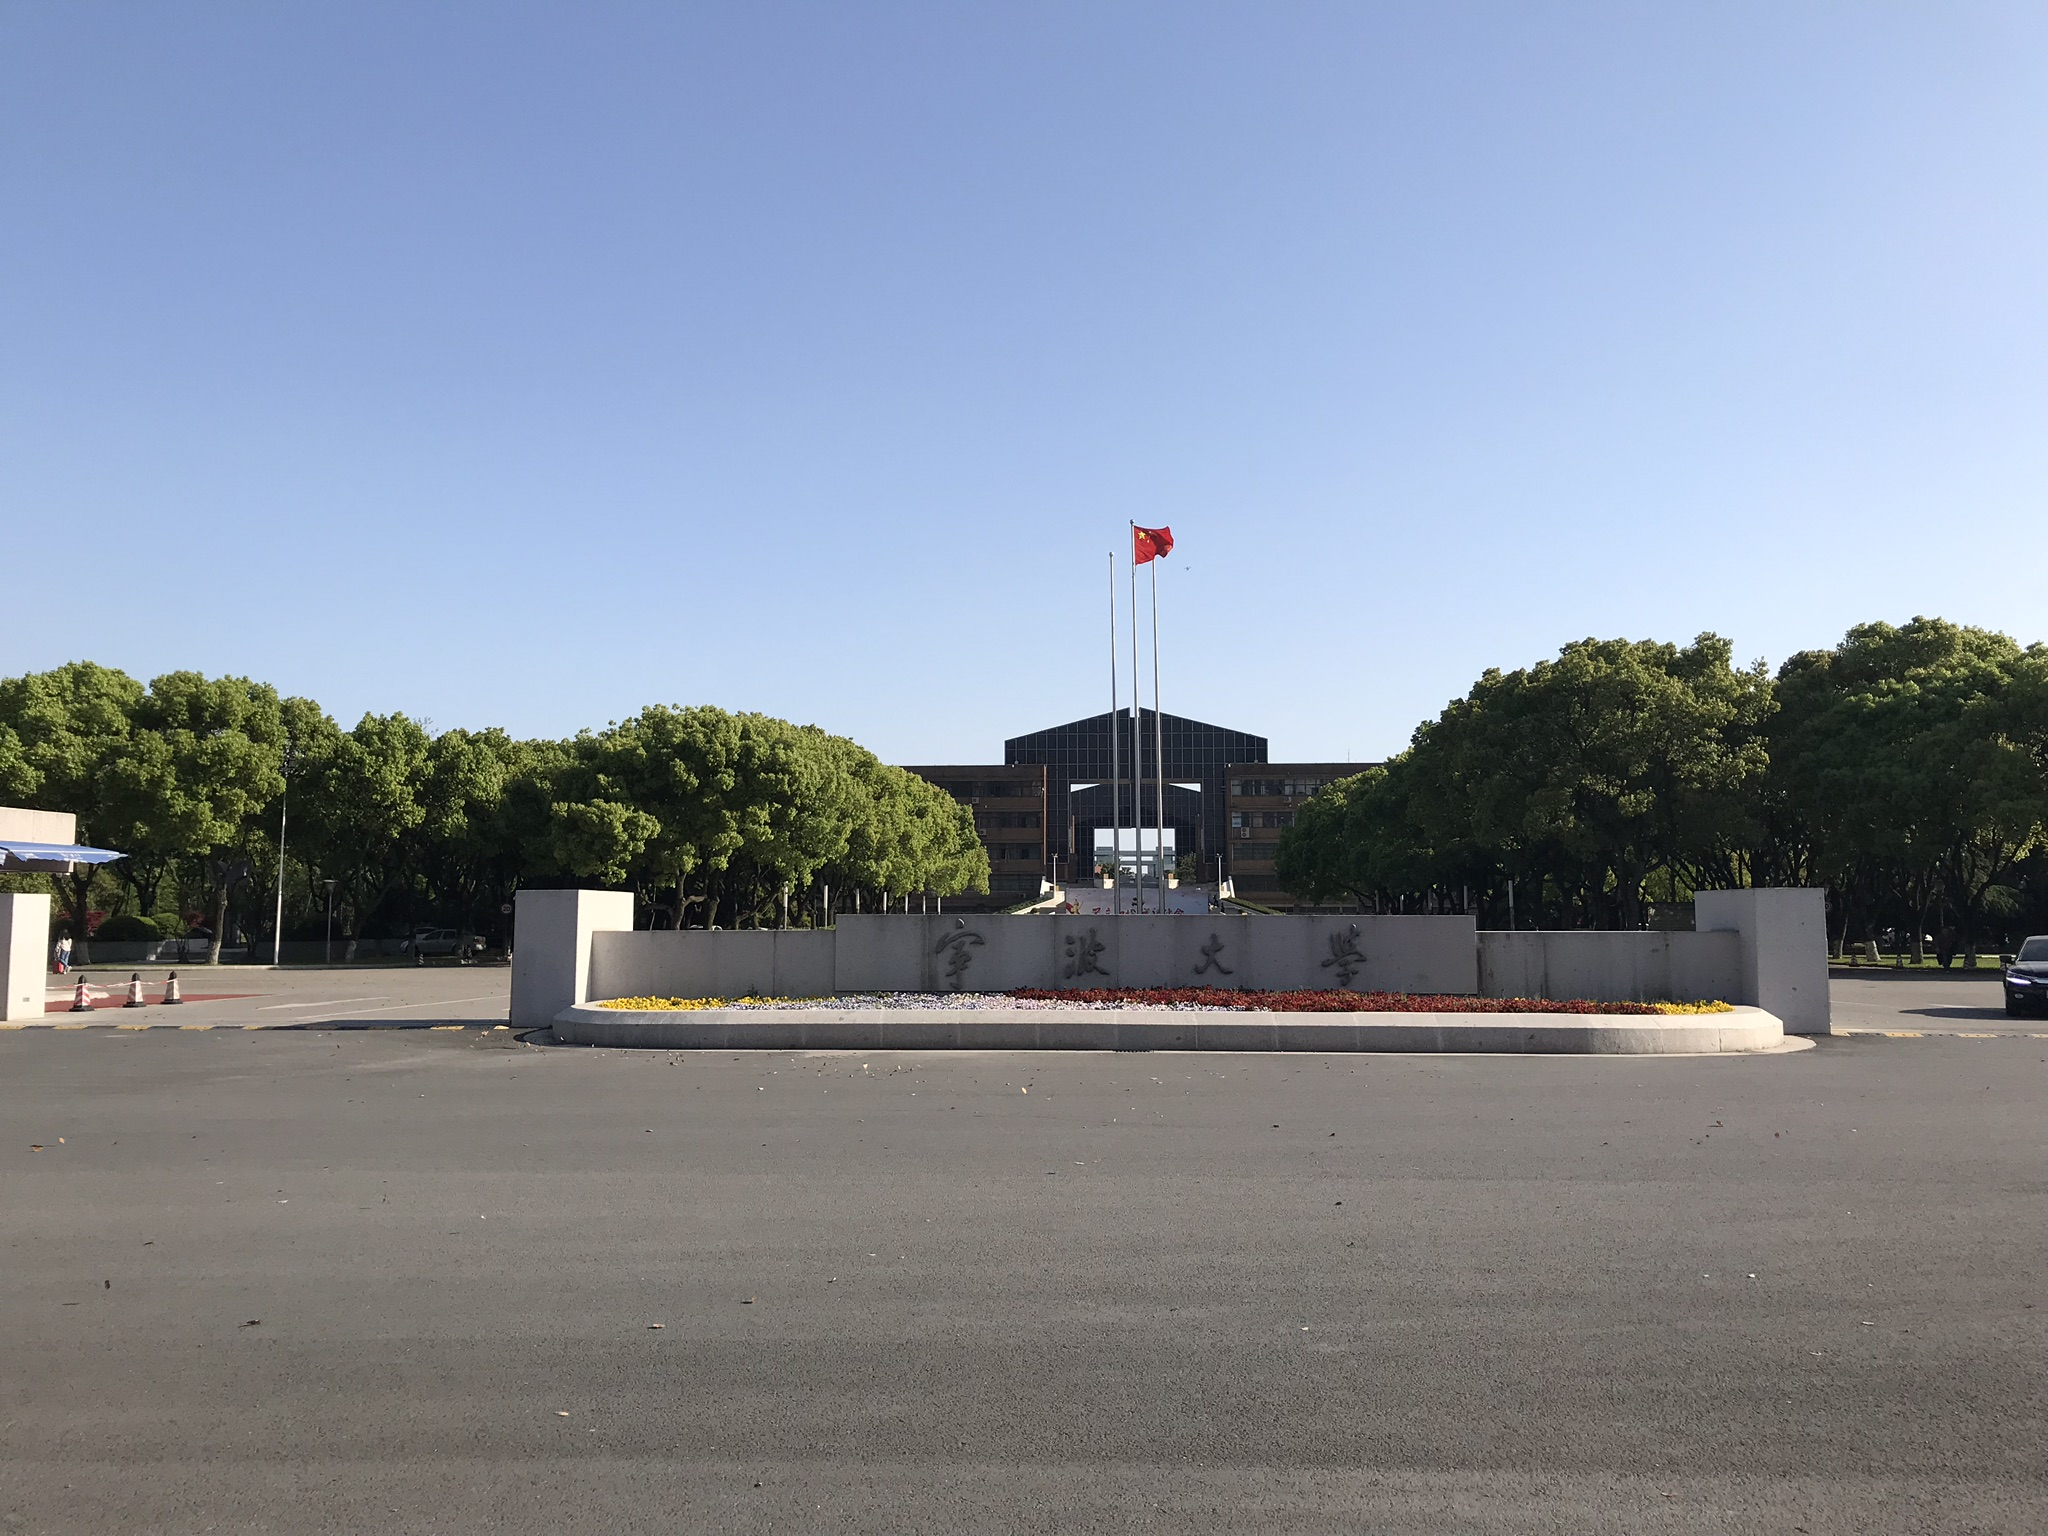
\includegraphics[width=0.82\textwidth]{figures/ningbo_university_gate.jpg}
  \caption{宁波大学正门示例图（图源：Nbfreeh，CC BY-SA 4.0，经 Wikimedia Commons）}
  \label{fig:ningbo-university-gate}
\end{figure}

\section{论文结构安排}
\label{sec:structure}

正文最多建议使用三级标题，即 \verb|\chapter|、\verb|\section| 和 \verb|\subsection|。目录默认显示到三级标题。若确有需要，可在本节中用列表概述各章职责，但不要手写章节编号。

% !TeX root = ../main.tex
\chapter{研究基础与问题建模}
\label{chap:foundation}

本章用于展示问题定义、公式、变量说明和交叉引用写法。正式论文中，应在公式前定义变量含义，并在公式后解释公式的作用，避免只堆叠符号。

\section{基本概念}
\label{sec:basic-concepts}

设源对象为 $M_s$，待比较对象为 $M_u$，审计样本集合为 $\mathcal{Q}=\{q_i\}_{i=1}^{N}$。这里的符号仅作为模板示例；正式写作时应替换为本研究的真实对象和变量。

\section{形式化目标}
\label{sec:formal-objective}

公式编号自动采用“章号.公式号”，例如式~\eqref{eq:sample-objective}。正文变量默认使用数学字体，不要把 Word 公式截图或公式对象残留复制到 TeX 源码中。

\begin{equation}
  S(M_u,M_s)=\frac{1}{N}\sum_{i=1}^{N}s\bigl(M_u(q_i),M_s(q_i)\bigr),
  \label{eq:sample-objective}
\end{equation}

其中，$S(M_u,M_s)$ 表示两个对象在审计样本集合上的平均相似度，$s(\cdot,\cdot)$ 表示单个样本上的评分函数。正式论文中，评分函数、阈值和样本来源均应给出清晰定义。

\subsection{三级标题示例}
\label{subsec:third-level-example}

三级标题用于功能性分段。若一个小节只有一两段文字，通常不需要继续拆分，以免目录碎片化。

% !TeX root = ../main.tex
\chapter{方法设计示例}
\label{chap:method-example}

本章展示方法章的常见写法：先说明设计动机，再给出流程、变量、组件和判别规则。正式论文中，每个模块都应回答“为什么这样设计、如何实现、输出是什么”。

\section{总体流程}
\label{sec:method-flow}

方法流程可以用段落、公式、图或算法描述。若使用图示，应确保图中术语与正文一致；若引用图，请使用自动编号，例如图~\ref{fig:ningbo-university-gate}。

\section{关键模块}
\label{sec:key-components}

下面的列表展示正文中枚举项的排版方式。列表应服务于论证，不宜替代连续分析。

\begin{enumerate}[label=\arabic*.]
  \item 数据准备：说明样本来源、筛选规则和划分方式。
  \item 特征构造：说明模型输入、输出和中间变量。
  \item 判别规则：说明评分函数、阈值选择和评价指标。
\end{enumerate}

% !TeX root = ../main.tex
\chapter{实验与结果展示示例}
\label{chap:experiment-example}

本章展示普通表格和复杂结果表的写法。正式论文中，实验章节应包括实验目标、设置、数据、指标、结果、分析和小结。没有真实实验日志时，不要填写虚构数值。

\section{实验设置}
\label{sec:experiment-setup}

表题格式由模板自动设置为“表章号-表号  表题”。普通表格默认使用五号字、1.5 倍行距和三线表风格。

\begin{table}[htbp]
  \centering
  \caption{实验设置字段示例}
  \label{tab:setup-example}
  \begin{tabular}{C{0.25\textwidth}P{0.55\textwidth}}
    \toprule
    项目 & 填写说明 \\
    \midrule
    数据集 & 写明数据来源、版本、样本数和划分方式。 \\
    模型 & 写明模型名称、版本、参数规模和来源。 \\
    指标 & 写明指标定义、统计单位和阈值选择方式。 \\
    \bottomrule
  \end{tabular}
\end{table}

\section{结果表格}
\label{sec:result-table}

复杂结果表可以调用 \verb|\nbucompacttable|，该命令只作用于下一张表格，适合列较多的实验结果。示例见表~\ref{tab:compact-result-example}。

% !TeX root = ../main.tex
% 复杂实验结果表例外：列较多时可在 table 内调用 \nbucompacttable，使表内字号和行距局部收紧。
\begin{table}[htbp]
  \centering
  \caption{复杂结果表占位示例}
  \label{tab:compact-result-example}
  \nbucompacttable
  \begin{tabular}{C{0.20\textwidth}C{0.16\textwidth}C{0.16\textwidth}C{0.16\textwidth}C{0.16\textwidth}}
    \toprule
    方法 & 指标一 & 指标二 & 指标三 & 备注 \\
    \midrule
    Baseline & -- & -- & -- & 替换为真实结果 \\
    Ours & -- & -- & -- & 替换为真实结果 \\
    \bottomrule
  \end{tabular}
\end{table}


% !TeX root = ../main.tex
\chapter{结论与展望}
\label{chap:conclusion}

结论章节应回到研究问题，概括本文已经完成的工作、证据支持的结论、方法局限和后续方向。结论中不要引入正文未报告的新实验或新数据。

\section{全文总结}
\label{sec:summary}

本节概括全文贡献。正式写作时，建议按“研究问题、方法设计、实验发现、论文贡献”的顺序组织，不使用夸张或无证据的评价词。

\section{研究展望}
\label{sec:future-work}

本节说明未来可继续改进的方向。展望应与本文局限直接对应，不宜泛泛而谈。


% 参考文献、致谢、附录均进入目录。
\printbibliography[heading=bibintoc,title={参考文献}]
\thesisacknowledgement{% !TeX root = ../main.tex
% 致谢应替换为作者自己的真实表达。模板不保留任何个人、导师、实验室或项目信息。
感谢在论文写作、学习和生活中给予帮助的师长、同学、朋友与家人。正式提交前，请根据个人实际情况重写本节，并避免包含不适合公开发布的隐私信息。
}
\appendix
\chapter*{附录}
\addcontentsline{toc}{chapter}{附录}
% !TeX root = ../main.tex
% 附录可放置补充证明、额外表格、实验配置、问卷、代码片段或数据说明。
本附录展示补充材料的写法。正式论文中，附录内容应与正文引用保持一致，并避免放入账号、绝对路径、未公开数据或其他敏感信息。


\end{document}
